
\medskip

Pour fabriquer un puits dans son jardin, M\up{me} Martin a besoin d'acheter 5 cylindres en
béton comme celui décrit ci-dessous.

Dans sa remorque, elle a la place pour mettre les 5 cylindres mais elle ne peut
transporter que $500$~kg au maximum.

À l'aide des caractéristiques du cylindre, déterminer le nombre minimum d'allers-retours
nécessaires à M\up{me} Martin pour rapporter ses 5 cylindres avec sa remorque.

\begin{tabularx}{\linewidth}{|m{0.4\textwidth} X|}\hline
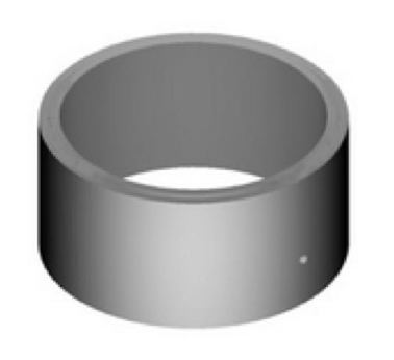
\includegraphics[width=5cm]{cylindre_Asie}&\textbf{Caractéristiques d'un cylindre }:

$\bullet~~$ diamètre intérieur: 90 cm

$\bullet~~$ diamètre extérieur: 101 cm

$\bullet~~$ hauteur: 50 cm

$\bullet~~$ masse volumique du béton: \np{2400} kg/m$^3$\\ \hline
\multicolumn{2}{|c|}{Rappel: volume d'un cylindre $= \pi  \times  \text{rayon} \times \text{rayon} \times \text{hauteur}$}\\
~\\\hline
\end{tabularx}

\bigskip

